\documentclass[aspectratio=169, 11pt]{beamer}

% ── Theme ────────────────────────────────────────────────────────────
\usetheme{Madrid}
\usecolortheme{whale}
\setbeamertemplate{navigation symbols}{}
\setbeamertemplate{footline}{%
  \leavevmode\hbox{%
    \begin{beamercolorbox}[wd=.33\paperwidth,ht=2.5ex,dp=1ex,center]{author in head/foot}%
      \usebeamerfont{author in head/foot}\insertshortauthor
    \end{beamercolorbox}%
    \begin{beamercolorbox}[wd=.34\paperwidth,ht=2.5ex,dp=1ex,center]{title in head/foot}%
      \usebeamerfont{title in head/foot}\insertshorttitle
    \end{beamercolorbox}%
    \begin{beamercolorbox}[wd=.33\paperwidth,ht=2.5ex,dp=1ex,right]{date in head/foot}%
      \usebeamerfont{date in head/foot}\insertframenumber{} / \inserttotalframenumber\hspace*{2ex}
    \end{beamercolorbox}%
  }%
}

% ── Packages ─────────────────────────────────────────────────────────
\usepackage{graphicx}
\usepackage{booktabs}
\usepackage{amsmath}
\usepackage{xcolor}
\usepackage{tikz}
\usepackage{pgfpages}

% Speaker notes on second screen (comment out for handout without notes)
\setbeameroption{show notes on second screen=right}

% ── Metadata ─────────────────────────────────────────────────────────
\title[Asymmetric Relation Dynamics]{Can Adding Asymmetric Relation Dynamics\\Make Knowledge Transfer More Efficient\\in Language Agents?}
\author[Rishi More]{Rishi More \texttt{(rmore2)}}
\institute[JHU]{EN.601.773 Machine Social Intelligence \\ Johns Hopkins University}
\date{Spring 2026}

\begin{document}

% =====================================================================
% TITLE
% =====================================================================
\begin{frame}
\titlepage
\note{
Hi everyone. Today I'll be presenting my project on whether asymmetric relational dynamics---like a caregiver-child structure---can make knowledge transfer more efficient in language agents. This is for the Machine Social Intelligence course.
}
\end{frame}

% =====================================================================
% MOTIVATION
% =====================================================================
\begin{frame}{Motivation}
\begin{columns}[T]
\column{0.55\textwidth}
\textbf{Human learning is relational}
\begin{itemize}
    \item Caregivers curate the information stream
    \item They highlight what is novel, correct misconceptions
    \item They adjust to the learner's current understanding
\end{itemize}

\vspace{0.5em}
\textbf{AI training ignores this}
\begin{itemize}
    \item No persistent teacher--learner relationship
    \item No selective attention or pedagogical framing
    \item No adaptive scaffolding
\end{itemize}

\column{0.42\textwidth}
\begin{block}{Research Question}
Does learning in an \textbf{asymmetric relational dynamic} enable a language agent to acquire richer and more generalizable knowledge than learning \textbf{alone} or from a \textbf{symmetric peer}?
\end{block}
\end{columns}

\note{
The motivation comes from developmental psychology. Humans don't learn in isolation---from birth, caregivers curate the information stream, selectively revealing what the child is ready to receive. This cooperative pedagogy is arguably the most efficient knowledge transfer mechanism in nature, but it's completely absent from how we train AI agents today.

So the research question is: if we give a language agent a persistent caregiver relationship, does it learn better than training alone or with a symmetric peer?
}
\end{frame}

% =====================================================================
% FRAMEWORK OVERVIEW
% =====================================================================
\begin{frame}{Framework Overview}
\begin{columns}[T]
\column{0.48\textwidth}
\textbf{Task Environment}
\begin{itemize}
    \item 197 procedural household tasks
    \item 10 categories, 8 difficulty levels
    \item 157 training / 40 held-out evaluation
    \item Multi-stage generation pipeline with Qwen3-235B + BM25 diversity filtering
\end{itemize}

\vspace{0.4em}
\textbf{Models}
\begin{itemize}
    \item \textbf{Caregiver}: Qwen3-235B (frozen)
    \item \textbf{Child}: Qwen3-8B + LoRA adapter
    \item \textbf{Judge}: 235B semantic action evaluator
\end{itemize}

\column{0.48\textwidth}
\textbf{Agent Memory Architecture}
\begin{enumerate}
    \item[\textbf{M1.}] \textbf{Instinct Buffer} -- Fixed system prompt (role priors)
    \item[\textbf{M2.}] \textbf{Working Memory} -- Last 8 dialogue turns
    \item[\textbf{M3.}] \textbf{Long-Term Memory} -- Episodic store with BM25 retrieval \& 235B compression
    \item[\textbf{M4.}] \textbf{Habit Store} -- LoRA weights updated via salience-weighted SFT
\end{enumerate}
\end{columns}

\note{
Here's the framework. On the left: I built a benchmark of 197 household tasks---things like cooking, cleaning, assembling furniture---spanning 8 difficulty levels. These were generated using a multi-stage pipeline with diversity filtering to avoid near-duplicate tasks.

The caregiver is a frozen 235B model that has access to the task solution. The child is an 8B model with a LoRA adapter that gets updated during training.

On the right is the memory architecture, inspired by cognitive science. Each agent has four memory systems: an instinct buffer that acts as a fixed system prompt, working memory for the last 8 turns, long-term episodic memory that stores compressed past experiences, and a habit store implemented as LoRA adapter weights.
}
\end{frame}

% =====================================================================
% SALIENCE SIGNAL
% =====================================================================
\begin{frame}{Salience-Gated Memory Consolidation}
\begin{block}{Salience Score}
\vspace{-0.5em}
\[
s = \underbrace{\alpha \cdot \text{novelty}(e)}_{\text{information-theoretic}} + \underbrace{\beta \cdot \text{prediction\_error}(e)}_{\text{Rescorla-Wagner + ZPD}} + \underbrace{\gamma \cdot \text{teaching}(e)}_{\text{productive struggle}}
\]
\end{block}

\vspace{0.3em}
\begin{columns}[T]
\column{0.32\textwidth}
\textbf{Novelty} ($\alpha{=}0.3$)
\begin{itemize}
    \footnotesize
    \item Category frequency decay: $\frac{1}{1+\text{count}}$
    \item BM25 distance to stored LTM entries
\end{itemize}

\column{0.32\textwidth}
\textbf{Prediction Error} ($\beta{=}0.4$)
\begin{itemize}
    \footnotesize
    \item Outcome surprise: $|r - \bar{r}_\text{cat}|$
    \item ZPD match: Gaussian at $r{=}0.5$
\end{itemize}

\column{0.32\textwidth}
\textbf{Teaching Signal} ($\gamma{=}0.3$)
\begin{itemize}
    \footnotesize
    \item Correction $\to$ improvement patterns
    \item Effort: turns used / max turns
    \item \textcolor{red}{$\gamma = 0$ without caregiver}
\end{itemize}
\end{columns}

\vspace{0.5em}
\centering
Episodes with $s > \tau = 0.3$ are stored in LTM; LoRA updates weighted by $s \times \text{partial\_credit}$

\note{
The key mechanism is the salience signal, which determines what gets remembered and how strongly habits are formed. It has three components.

Novelty rewards new categories and tasks dissimilar to what's already in memory. Prediction error captures outcome surprise---using a Rescorla-Wagner model---and also ZPD matching, which prioritizes episodes that were neither too easy nor too hard. The teaching signal captures productive struggle: patterns where the caregiver corrected the child and the child then improved.

Critically, in the non-caregiver conditions, gamma is set to zero---there's no teaching signal. This is the key manipulation that distinguishes our Relational condition.

Episodes above the salience threshold get stored in long-term memory, and LoRA updates are weighted by salience times partial credit.
}
\end{frame}

% =====================================================================
% ADAPTIVE SCAFFOLDING
% =====================================================================
\begin{frame}{Adaptive Scaffolding}
\begin{columns}[T]
\column{0.55\textwidth}
\textbf{Caregiver adjusts support based on child competence:}

\vspace{0.5em}
\begin{tabular}{ll}
\toprule
\textbf{Competence} & \textbf{Scaffolding Level} \\
\midrule
$< 0.3$ & Full support (step-by-step) \\
$0.3$--$0.7$ & Guided discovery (questions) \\
$> 0.7$ & Minimal support (brief cues) \\
\bottomrule
\end{tabular}

\vspace{0.5em}
\begin{itemize}
    \item Competence = rolling avg of partial credit over last 5 episodes per category
    \item Implements Vygotsky's Zone of Proximal Development
\end{itemize}

\column{0.42\textwidth}
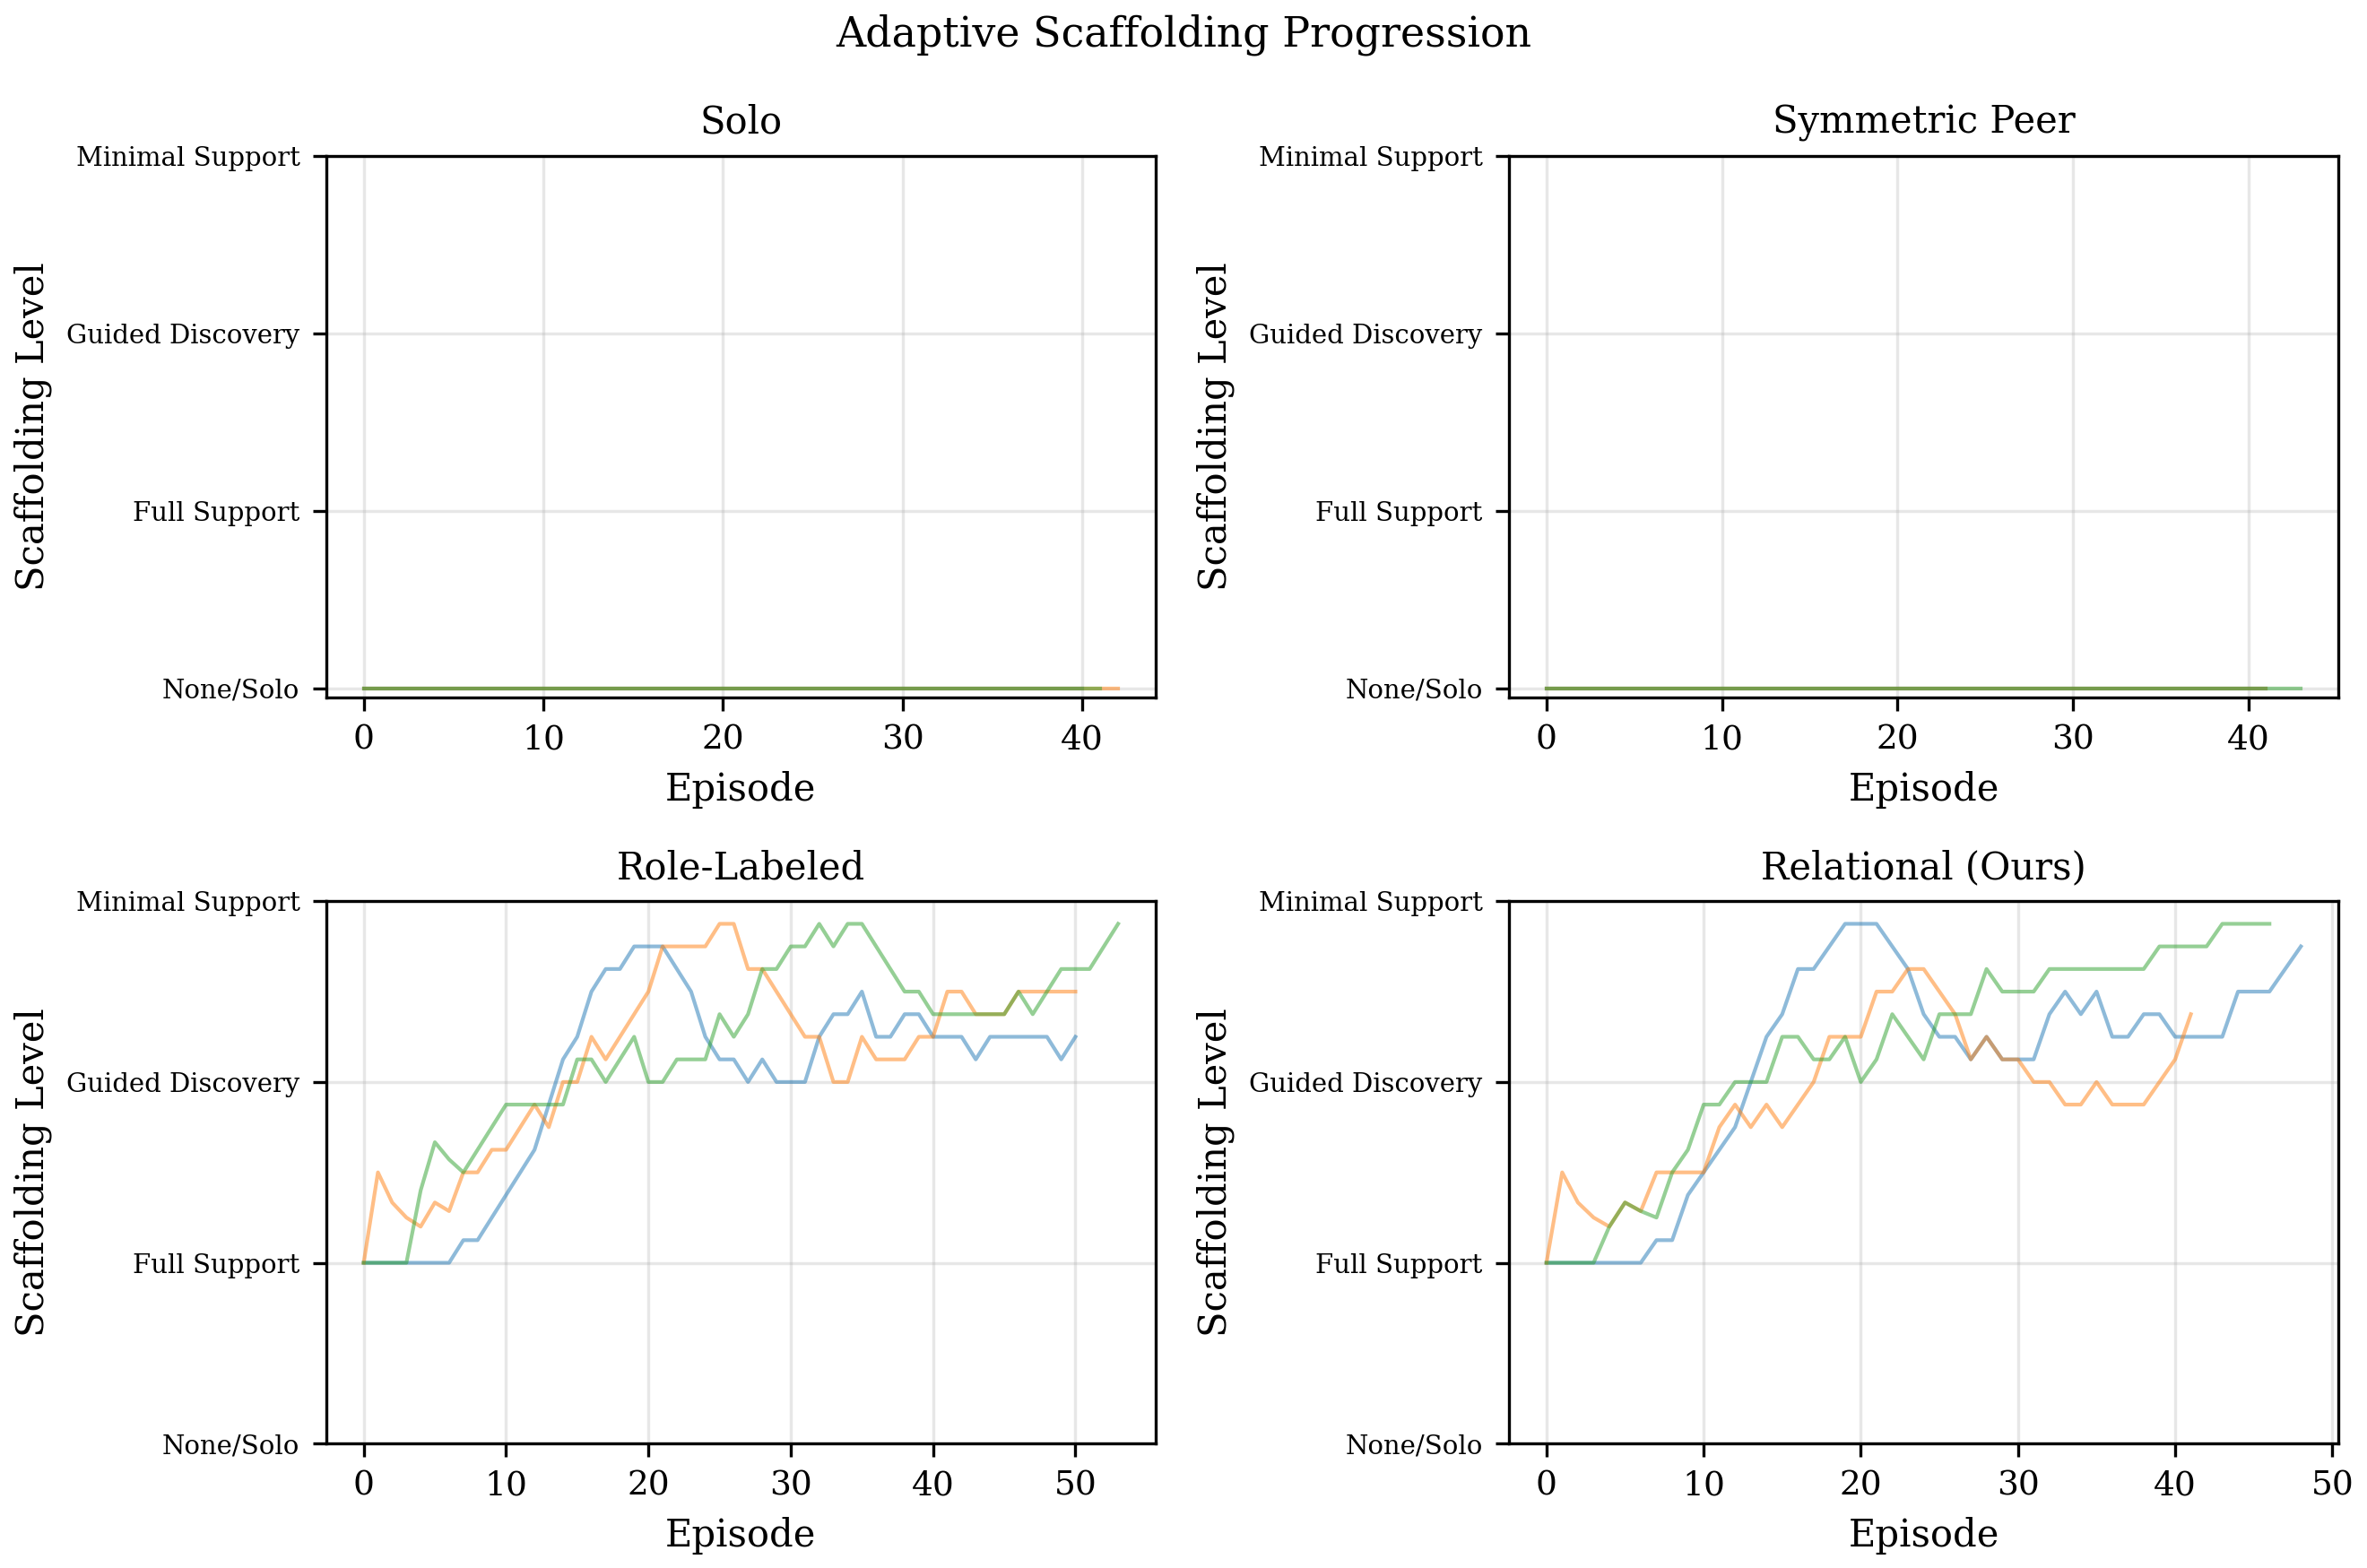
\includegraphics[width=\textwidth]{figures/competence_levels.png}
\end{columns}

\note{
The caregiver doesn't just give the same level of help throughout. It tracks the child's competence per category using a rolling average of partial credit scores. When competence is low, it gives full step-by-step instructions. As the child improves, it transitions to asking guiding questions, and eventually just gives brief confirmations.

The figure on the right shows how this plays out---you can see the scaffolding level increasing over episodes, especially for the caregiver conditions.

This is inspired by Vygotsky's Zone of Proximal Development---the idea that teaching should target what the learner can almost do independently.
}
\end{frame}

% =====================================================================
% EXPERIMENTAL CONDITIONS
% =====================================================================
\begin{frame}{Experimental Conditions}
\begin{table}
\centering
\small
\begin{tabular}{p{2.5cm}p{3.8cm}p{5.5cm}}
\toprule
\textbf{Condition} & \textbf{Agent Structure} & \textbf{Key Difference} \\
\midrule
Solo & Single 8B child & No partner; $\gamma = 0$ \\
Symmetric Peer & Two 8B agents & Both are ``children''; $\gamma = 0$ \\
Role-Labeled & 235B caregiver + 8B child & Asymmetric prompts; $\gamma = 0$ \\
\textbf{Relational} & 235B caregiver + 8B child & \textbf{Full salience with $\gamma = 0.3$} \\
\bottomrule
\end{tabular}
\end{table}

\vspace{0.5em}
\begin{itemize}
    \item 4 conditions $\times$ 3 seeds = \textbf{12 concurrent runs}
    \item 160 episodes each, curriculum ordered by difficulty
    \item Shared frozen 235B caregiver across all runs
    \item Fully async pipeline via \texttt{asyncio} for max API throughput
\end{itemize}

\note{
Here are the four conditions. Solo is just the child alone. Symmetric Peer has two 8B models interacting without role asymmetry. Role-Labeled gives the child a 235B caregiver but without the teaching signal in salience. And Relational is our full condition with the teaching signal turned on.

The Role-Labeled vs Relational comparison isolates whether the teaching signal in memory consolidation matters beyond just having a good teacher present.

We ran 12 concurrent training runs---all sharing a single frozen 235B caregiver client---using asyncio for maximum API throughput. Each run goes through 160 episodes ordered by difficulty.
}
\end{frame}

% =====================================================================
% HYPOTHESES
% =====================================================================
\begin{frame}{Research Hypotheses}
\begin{enumerate}
    \item[\textbf{H1.}] \textbf{Better memory}: The relational condition will produce higher transfer accuracy on held-out tasks

    \vspace{0.5em}
    \item[\textbf{H2.}] \textbf{Habit acceleration}: LoRA habits will form in fewer episodes with caregiver guidance

    \vspace{0.5em}
    \item[\textbf{H3.}] \textbf{Theory of Mind proxy}: The child will internalize the caregiver's pedagogical model (measured via dialogue prediction)
\end{enumerate}

\note{
We had three hypotheses. H1: the relational condition should produce better transfer to novel tasks. H2: habits should form faster with caregiver guidance. And H3: the child should develop a theory of mind of the caregiver, measured by its ability to predict what the caregiver would say next.

Let's see what actually happened.
}
\end{frame}

% =====================================================================
% RESULTS: LEARNING CURVES
% =====================================================================
\begin{frame}{Results: Learning Curves During Training}
\begin{columns}[T]
\column{0.55\textwidth}
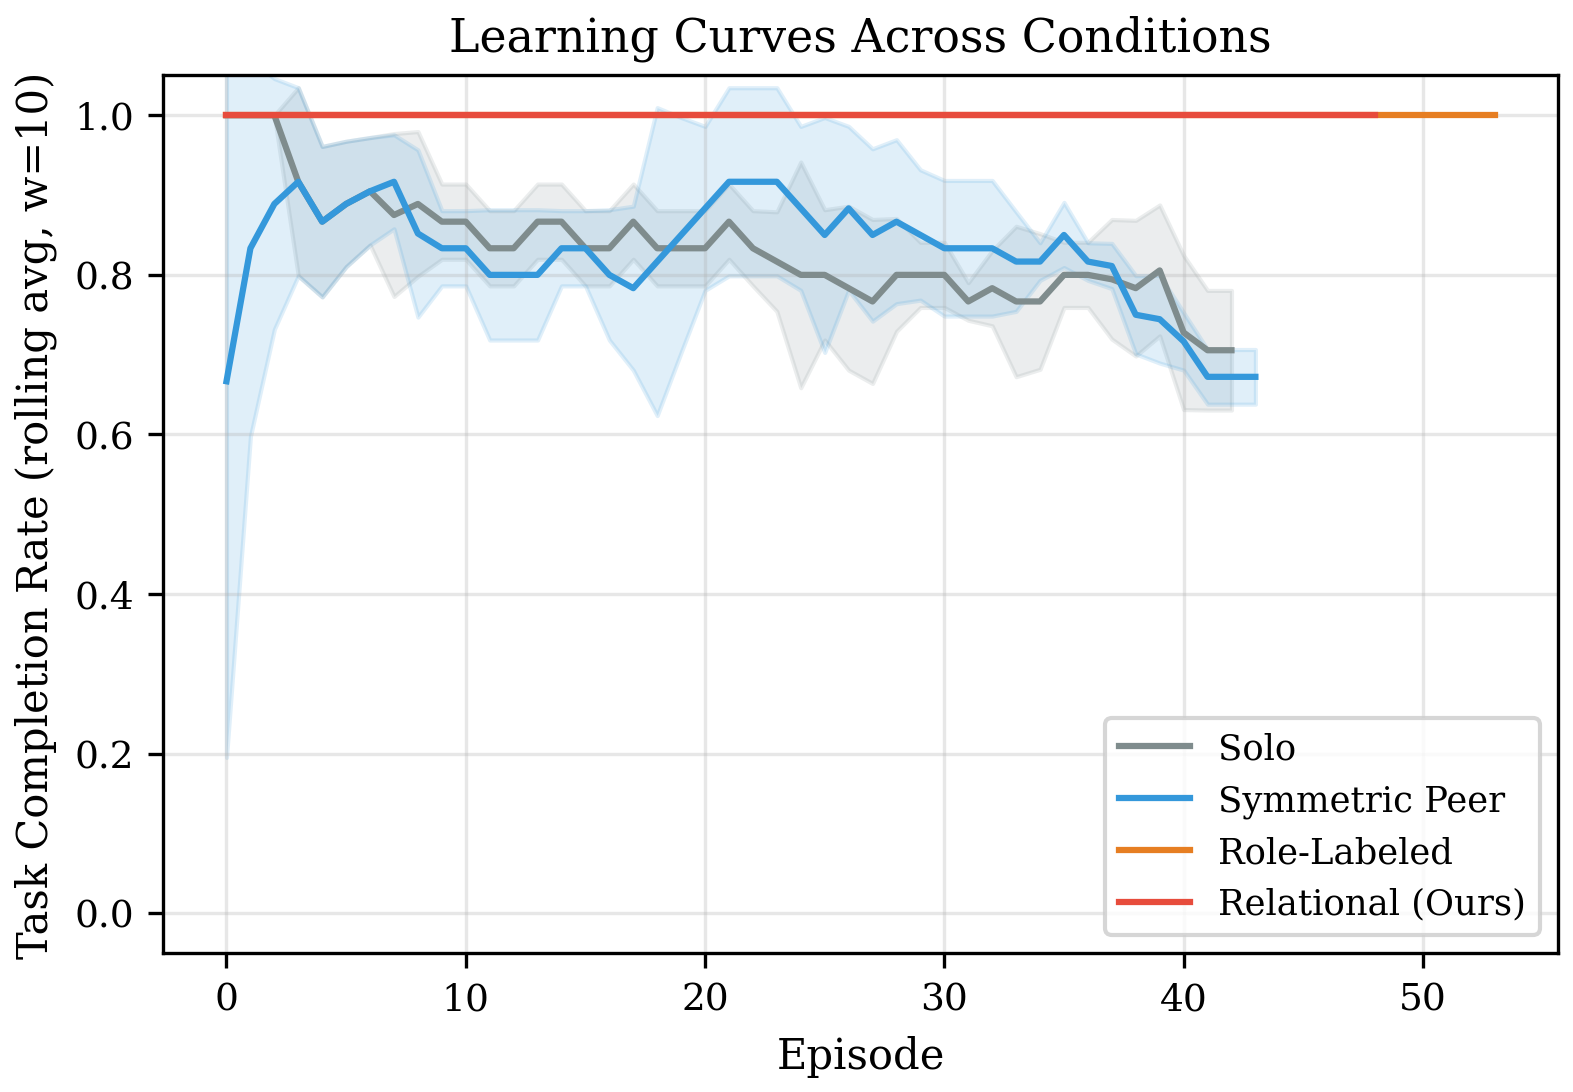
\includegraphics[width=\textwidth]{figures/learning_curves.png}

\column{0.42\textwidth}
\vspace{1em}
\textbf{Key observations:}
\begin{itemize}
    \item All conditions start well on easy tasks
    \item Solo \& Peer \textbf{degrade} as difficulty increases
    \item Caregiver conditions \textbf{maintain} near-perfect performance
    \item The caregiver fills knowledge gaps in real time
\end{itemize}
\end{columns}

\note{
Let's start with the learning curves. This shows the rolling average task completion rate over training episodes. The x-axis is episodes, and remember the curriculum gets harder over time.

All four conditions start well on easy tasks in the first 40 episodes. But as difficulty increases, Solo and Peer performance drops significantly---they can't figure out the harder multi-step tasks on their own. The caregiver conditions stay near perfect because the 235B model fills in the child's knowledge gaps in real time.

This is a dramatic training-time difference. But the question is: does this translate to better independent performance?
}
\end{frame}

% =====================================================================
% RESULTS: H2 TRAINING SUCCESS
% =====================================================================
\begin{frame}{Results: H2 -- Habit Acceleration}
\centering
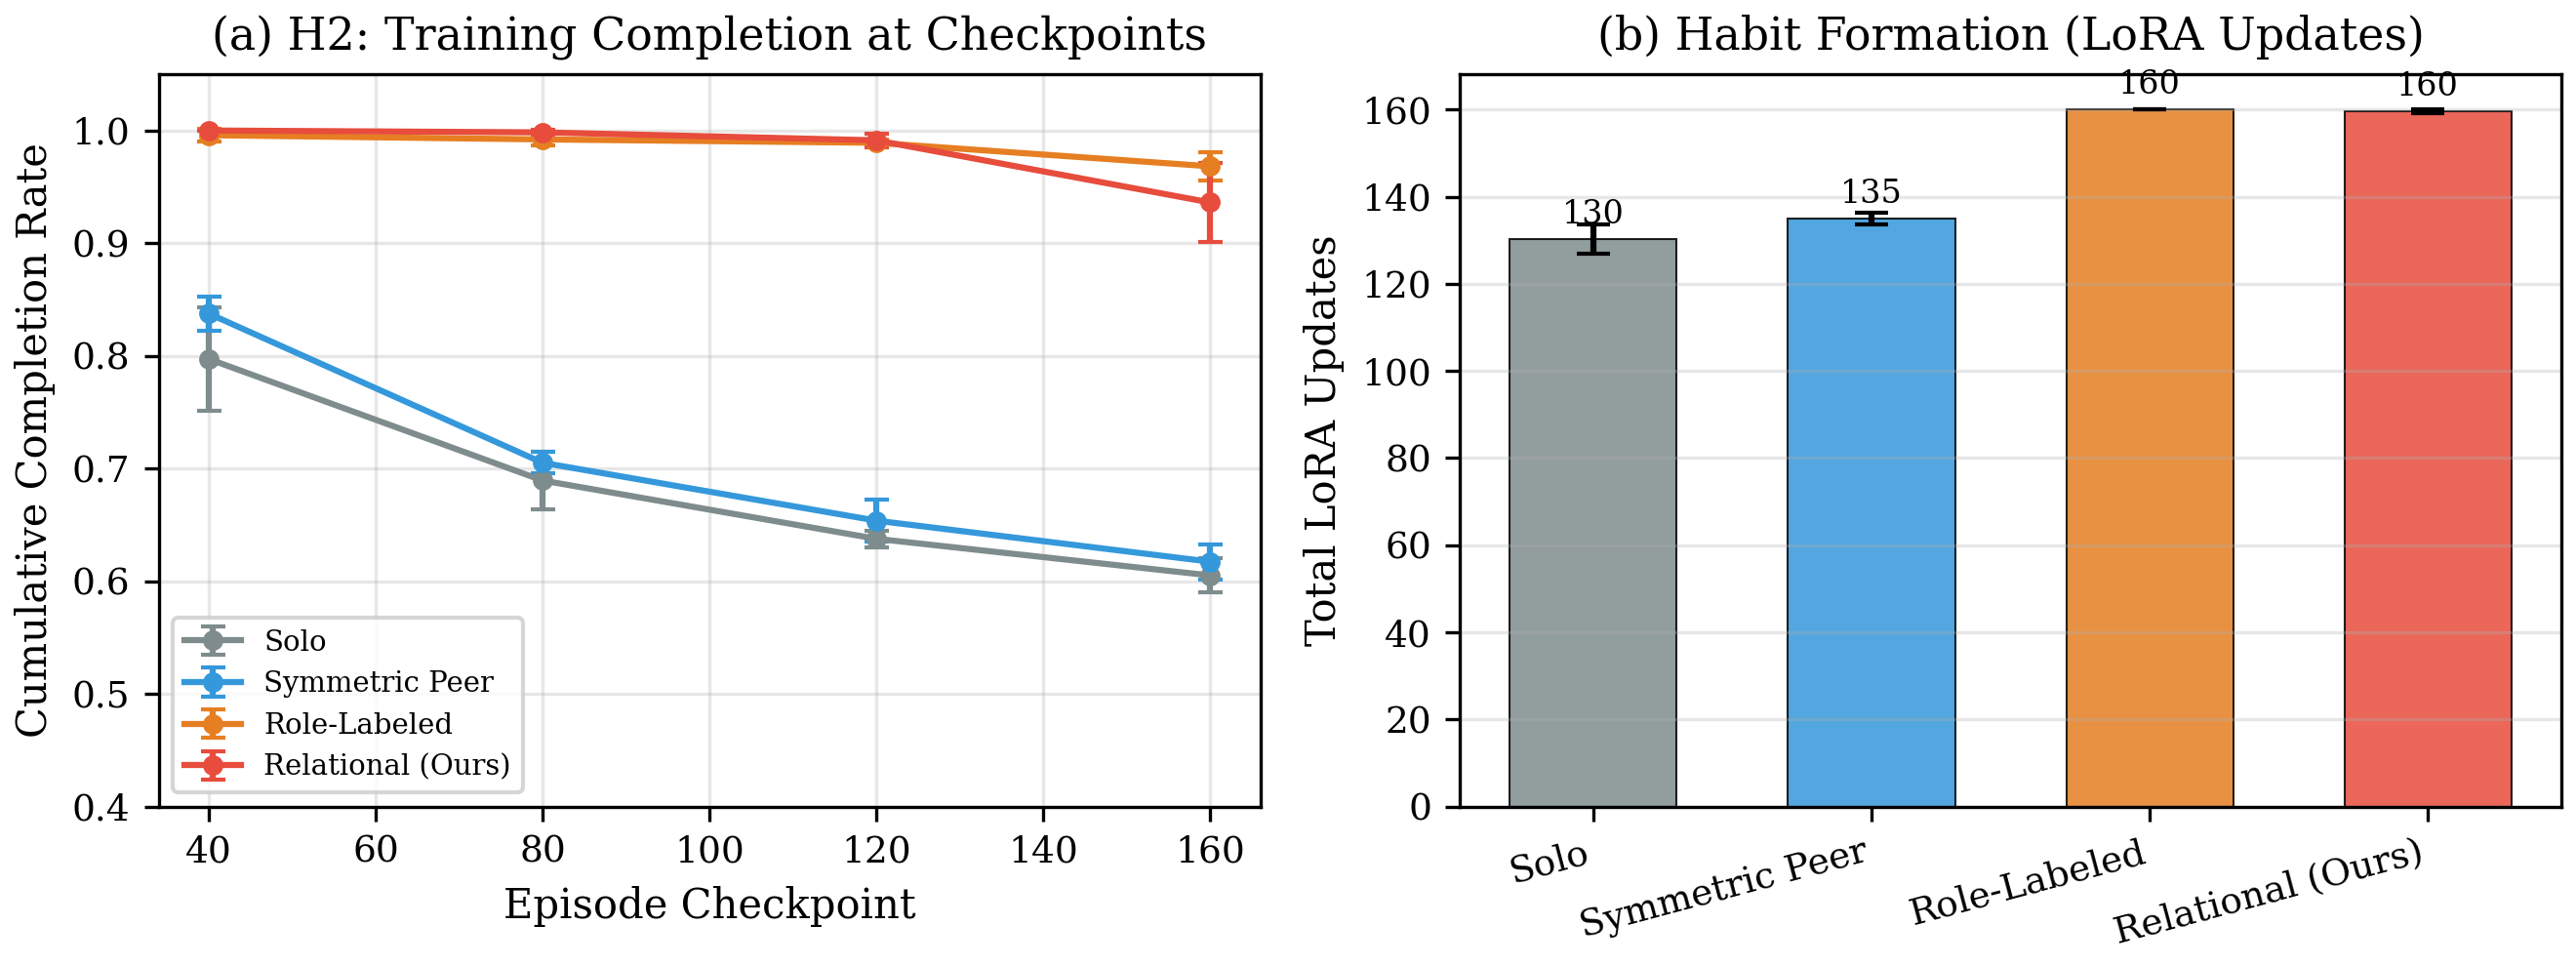
\includegraphics[width=0.85\textwidth]{figures/training_success.png}

\vspace{0.3em}
\small
Caregiver conditions: \textbf{100\% success}, 160 LoRA updates \quad vs. \quad Solo/Peer: \textbf{82--84\%}, $\sim$130 updates

\note{
This figure shows H2, the habit acceleration hypothesis. On the left, cumulative completion rate at training checkpoints. On the right, total LoRA updates.

The caregiver conditions achieve essentially perfect training success---every single episode results in a successful trajectory that gets encoded into LoRA weights. Solo and Peer only succeed on about 82-84 percent of episodes, and that rate drops as tasks get harder.

This is a genuine habit acceleration effect. The caregiver ensures the child always produces correct trajectories, so habit formation is continuous rather than intermittent. H2 is strongly supported.
}
\end{frame}

% =====================================================================
% RESULTS: TEACHING EFFICIENCY
% =====================================================================
\begin{frame}{Results: Teaching Efficiency}
\centering
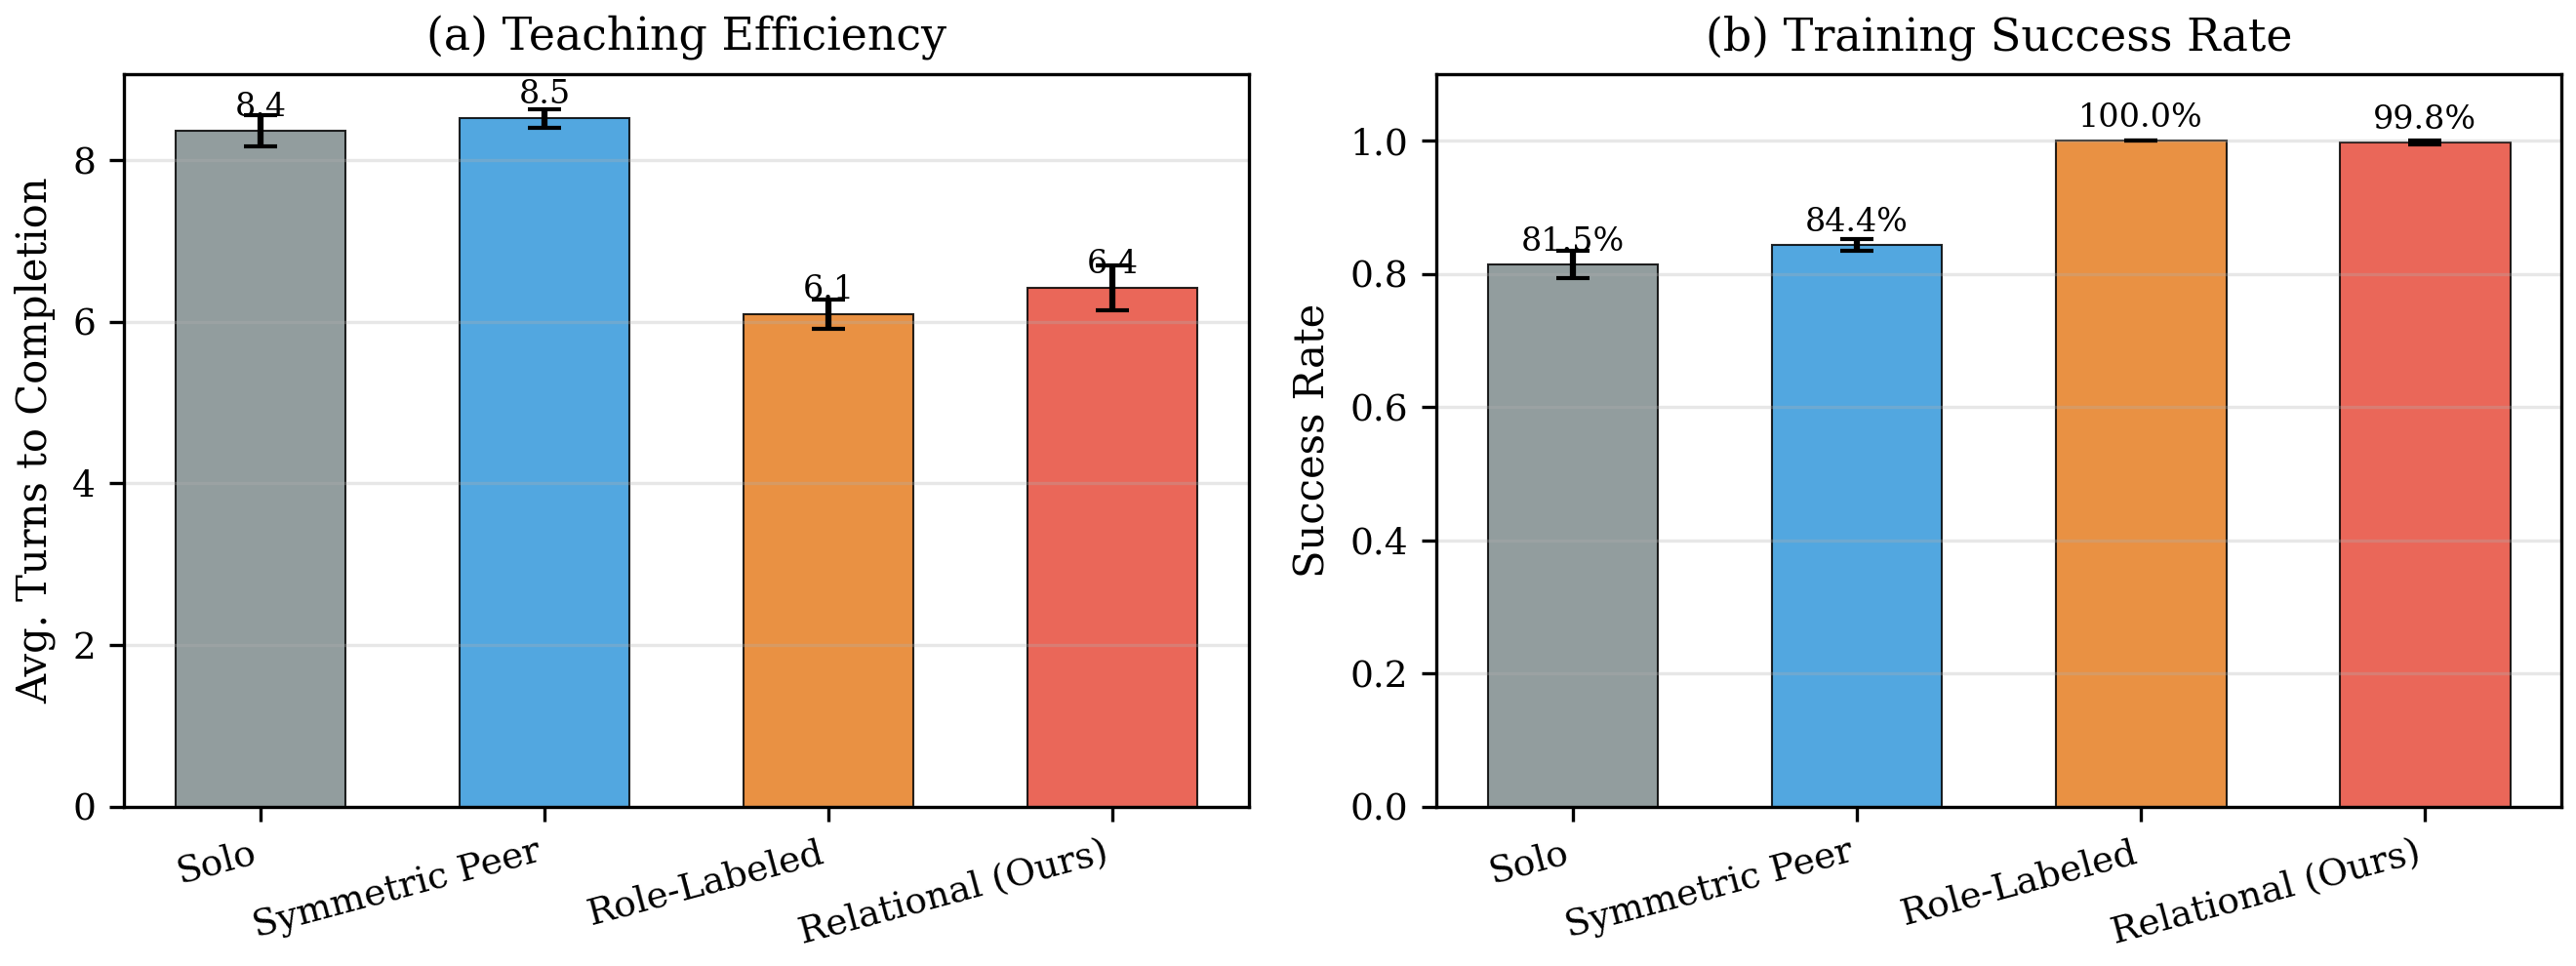
\includegraphics[width=0.85\textwidth]{figures/teaching_efficiency.png}

\vspace{0.3em}
\small
Caregiver: \textbf{6.1--6.4 turns} \quad vs. \quad Solo/Peer: \textbf{8.4--8.5 turns} \quad (\textbf{25\% reduction})

\note{
Teaching efficiency tells a similar story. The caregiver conditions complete tasks in about 6.1 to 6.4 turns on average, compared to 8.4 to 8.5 for Solo and Peer. That's a 25 percent reduction in dialogue turns.

Combined with the near-perfect success rate, this means the caregiver conditions extract substantially more learning signal per API call. They're both more effective and more efficient.
}
\end{frame}

% =====================================================================
% RESULTS: H1 TRANSFER
% =====================================================================
\begin{frame}{Results: H1 -- Transfer to Held-Out Tasks}
\begin{columns}[T]
\column{0.48\textwidth}
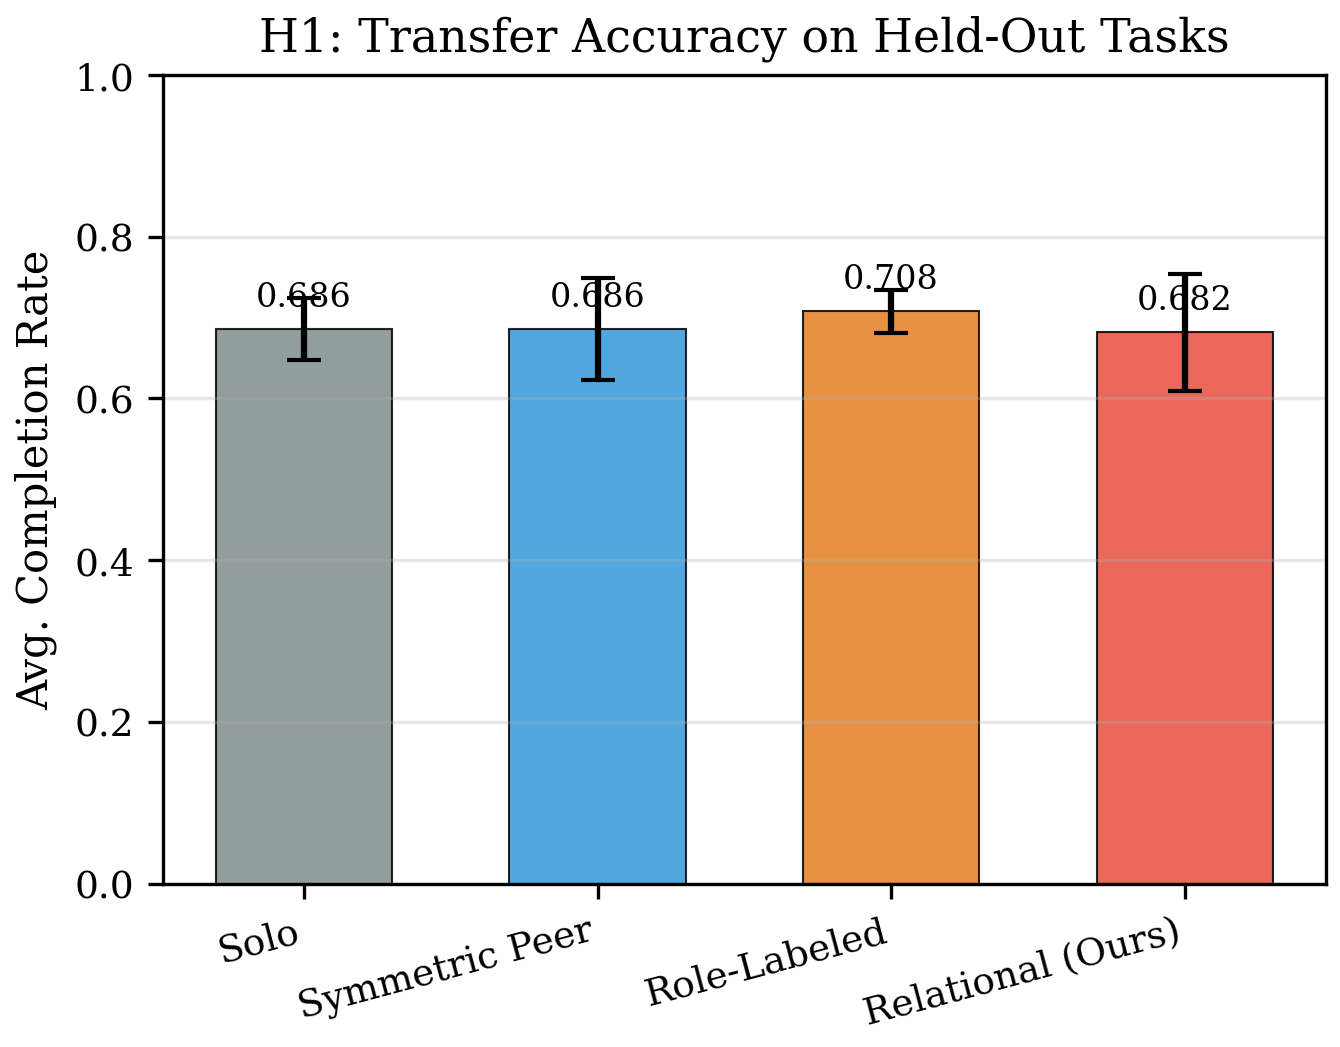
\includegraphics[width=\textwidth]{figures/h1_transfer.png}

\column{0.48\textwidth}
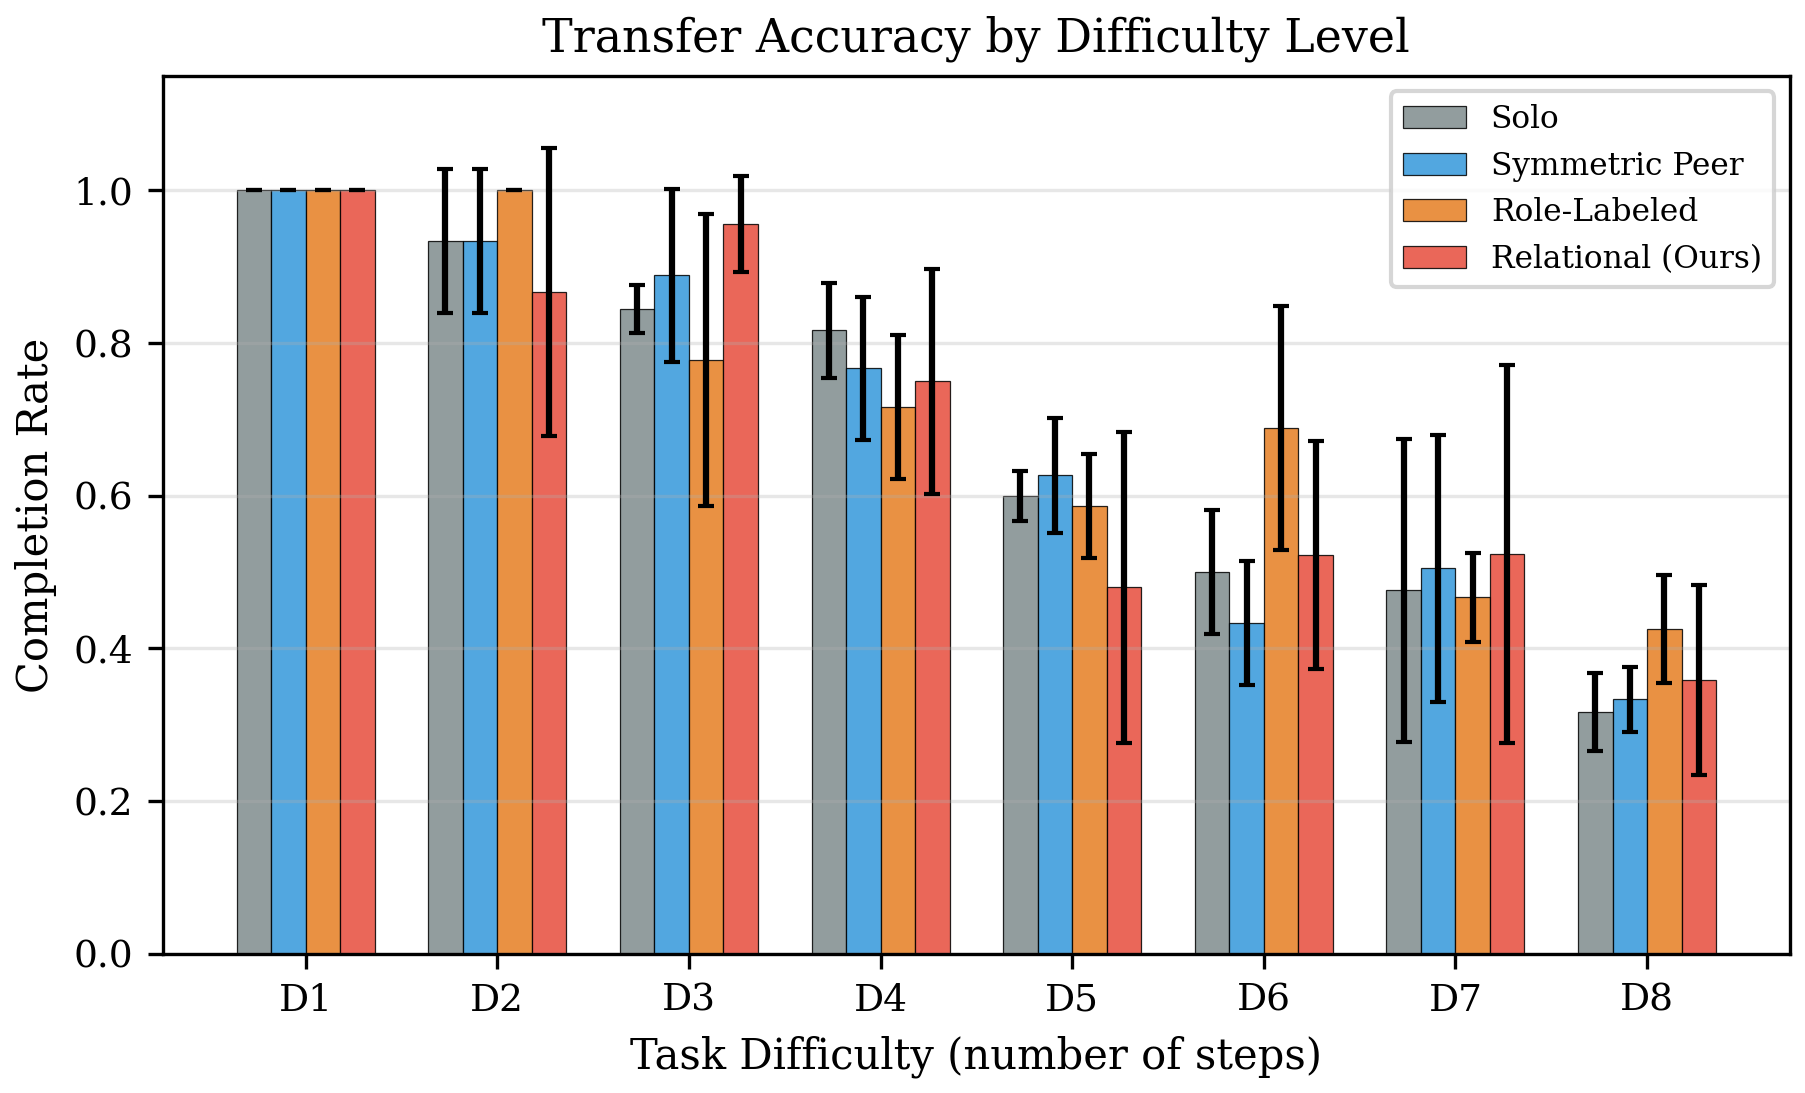
\includegraphics[width=\textwidth]{figures/transfer_by_difficulty.png}
\end{columns}

\vspace{0.3em}
\centering
\begin{tabular}{lccc}
\toprule
\textbf{Condition} & \textbf{Transfer Accuracy} \\
\midrule
Solo & $0.686 \pm 0.046$ \\
Peer & $0.686 \pm 0.078$ \\
Role-Labeled & $0.708 \pm 0.033$ \\
Relational & $0.682 \pm 0.087$ \\
\bottomrule
\end{tabular}

\note{
Now here's the surprise. H1 tested transfer accuracy on 40 held-out tasks where the child works alone---no caregiver help. And all four conditions perform essentially the same, around 0.68 to 0.71.

Despite the massive training-time advantage, the caregiver-trained agents do NOT transfer better to independent evaluation. The right panel breaks this down by difficulty, and there's no consistent advantage at any difficulty level.

This is our most interesting finding, and it leads directly to our main discussion point.
}
\end{frame}

% =====================================================================
% RESULTS: CATEGORY HEATMAP
% =====================================================================
\begin{frame}{Results: Category-Level Transfer}
\centering
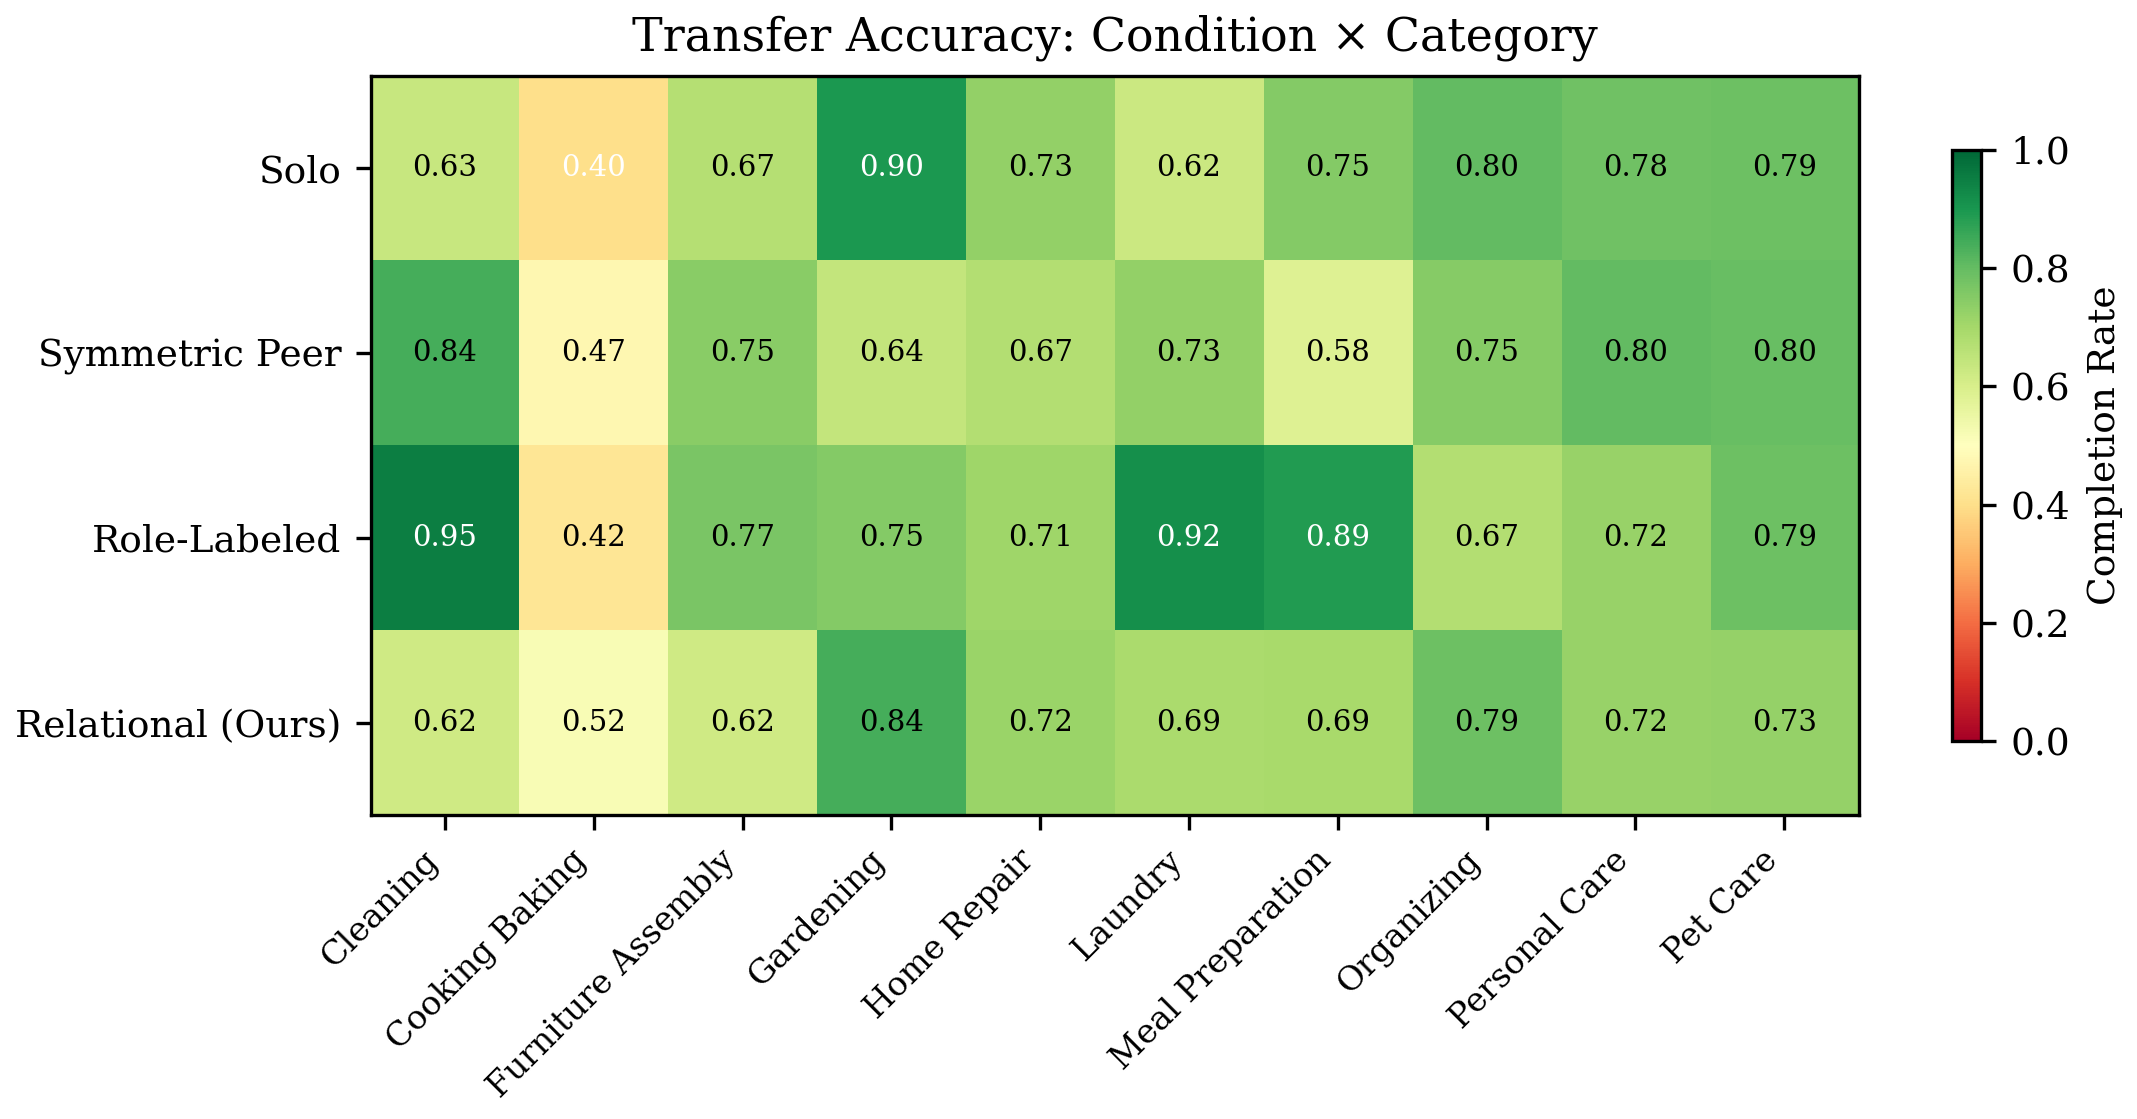
\includegraphics[width=0.75\textwidth]{figures/category_heatmap.png}

\vspace{0.3em}
\small
Task difficulty is category-dependent; no condition dominates across all categories

\note{
This heatmap shows transfer accuracy broken down by condition and task category. Some categories like pet care and meal preparation are consistently easier. Others like cleaning and cooking are harder across the board.

But no single condition dominates all categories---it's quite mixed. This is consistent with the overall H1 finding that the conditions produce similar transfer performance.
}
\end{frame}

% =====================================================================
% SCAFFOLDING DEPENDENCY
% =====================================================================
\begin{frame}{The Scaffolding Dependency Effect}
\begin{columns}[T]
\column{0.55\textwidth}
\begin{block}{The Central Finding}
Caregiver-assisted agents \textbf{dramatically outperform} during training but show \textbf{no transfer advantage} when tested independently.
\end{block}

\vspace{0.5em}
\textbf{Why?}
\begin{itemize}
    \item LoRA weights encode behaviors optimized for the \emph{assisted} context
    \item Without real-time corrective feedback, performance reverts
    \item Mirrors \textbf{scaffolding dependency} in developmental psychology (Wood et al., 1976)
\end{itemize}

\column{0.42\textwidth}
\vspace{1em}
\textbf{Missing ingredient:}
\begin{alertblock}{Scaffolding Fading}
The caregiver should \textbf{progressively withdraw} support, forcing the child to develop independent strategies.
\end{alertblock}

\vspace{0.5em}
\small
Our adaptive scaffolding reduces hint specificity but \textbf{never fully withdraws}---even ``minimal support'' still provides feedback every turn.
\end{columns}

\note{
This is our central finding and I think the most interesting result. There's a striking dissociation: 100 percent training success but no transfer advantage.

This directly mirrors a well-documented phenomenon in developmental psychology called scaffolding dependency. Vygotsky predicted that scaffolding should produce independent competence, but empirical studies show that learners can become dependent on external support if it's not systematically faded.

In our experiment, the 235B caregiver provides consistent guidance throughout all 160 episodes. The child learns to succeed WITH this support, and the LoRA weights encode behaviors optimized for the assisted context. When you remove the caregiver at evaluation time, that support structure disappears and performance reverts.

The missing ingredient is scaffolding fading---the caregiver should progressively withdraw, forcing the child to develop independent problem-solving. Our adaptive scaffolding reduces hint specificity but never fully withdraws.
}
\end{frame}

% =====================================================================
% ROLE ASYMMETRY vs RELATIONAL SALIENCE
% =====================================================================
\begin{frame}{Role Asymmetry vs.\ Relational Salience}
\begin{columns}[T]
\column{0.55\textwidth}
Role-Labeled and Relational perform \textbf{nearly identically}:

\vspace{0.5em}
\begin{tabular}{lcc}
\toprule
& \textbf{Role-Lab} & \textbf{Relational} \\
\midrule
Training success & 100\% & 99.8\% \\
Avg turns & 6.10 & 6.42 \\
Transfer H1 & 0.708 & 0.682 \\
LoRA updates & 160 & 159.7 \\
\bottomrule
\end{tabular}

\vspace{0.5em}
$\Rightarrow$ \textbf{Prompt-based role asymmetry} captures most of the benefit

\column{0.42\textwidth}
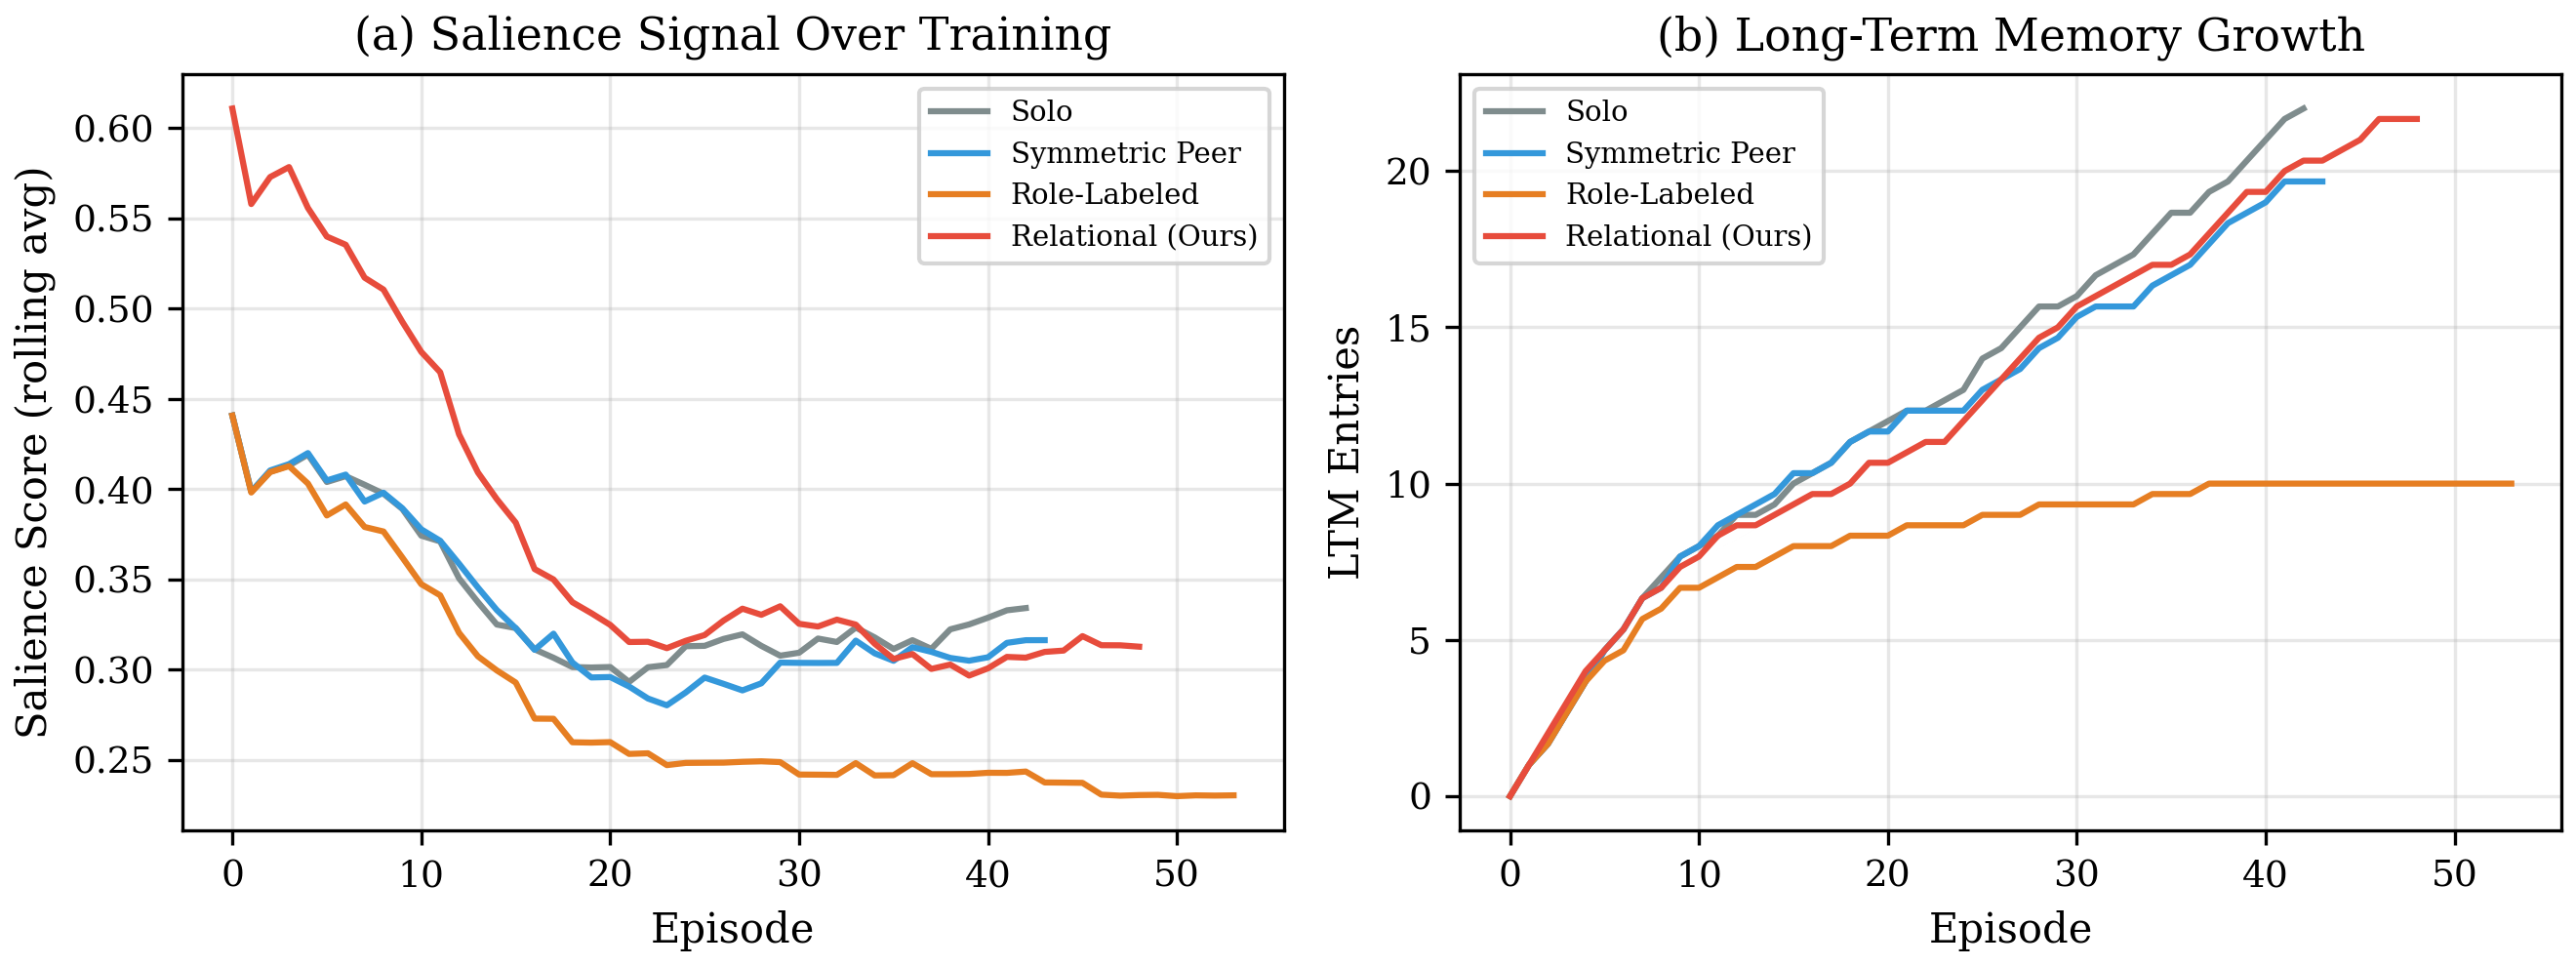
\includegraphics[width=\textwidth]{figures/salience_ltm.png}

\vspace{0.3em}
\small
Similar salience decay and LTM growth across both caregiver conditions
\end{columns}

\note{
Another finding: Role-Labeled and Relational performed nearly identically. This means that prompt-based role asymmetry---simply giving one agent a caregiver prompt and the other a child prompt---captures most of the benefit. The additional teaching signal in the salience score provides marginal improvement at best.

The salience and LTM growth curves on the right show very similar patterns for both caregiver conditions. This suggests the benefit of relational context is primarily in the caregiver's real-time guidance, not in how experiences are consolidated into memory.
}
\end{frame}

% =====================================================================
% H3 and LIMITATIONS
% =====================================================================
\begin{frame}{H3: Theory of Mind \& Limitations}
\begin{columns}[T]
\column{0.55\textwidth}
\textbf{H3 Result: Negative}
\begin{itemize}
    \item BM25 similarity between predicted and actual caregiver responses: \textbf{0.066 $\pm$ 0.003}
    \item Child did not meaningfully predict caregiver behavior
\end{itemize}

\vspace{0.5em}
\textbf{But: likely a measurement issue}
\begin{itemize}
    \item BM25 measures \emph{lexical} overlap
    \item ``What should we do first?'' vs.\ ``Remember the safety step'' $\to$ same intent, zero overlap
    \item Need embedding-based or model-based semantic similarity
\end{itemize}

\column{0.42\textwidth}
\textbf{Other Limitations}
\begin{itemize}
    \item Runs completed 41--54 of 160 planned episodes (API rate limits)
    \item 8B child with LoRA rank 16 has limited capacity for ToM
    \item Text-only environment lacks grounded perception
    \item Single caregiver personality
\end{itemize}
\end{columns}

\note{
H3 asked whether the child internalizes a model of the caregiver's pedagogy. We measured this by asking the child to predict what the caregiver would say next, then computing BM25 similarity. The score was near zero---0.066.

But I think this is mostly a measurement artifact. BM25 measures word overlap, and two semantically equivalent teaching utterances might share no keywords at all. A proper evaluation would need embedding-based or model-based semantic similarity.

On the right are other limitations. Due to API rate limits, our runs completed about 41 to 54 episodes out of 160 planned. The 8B model with LoRA rank 16 may simply lack the capacity for emergent Theory of Mind. And we only tested with a single caregiver personality.
}
\end{frame}

% =====================================================================
% SUMMARY TABLE
% =====================================================================
\begin{frame}{Summary of Results}
\centering
\begin{tabular}{lcccc}
\toprule
\textbf{Metric} & \textbf{Solo} & \textbf{Peer} & \textbf{Role-Lab} & \textbf{Relational} \\
\midrule
H1 Transfer & 0.686 & 0.686 & \textbf{0.708} & 0.682 \\
Train Success & 81.5\% & 84.4\% & \textbf{100\%} & 99.8\% \\
Avg Turns & 8.36 & 8.52 & \textbf{6.10} & 6.42 \\
LoRA Updates & 130 & 135 & \textbf{160} & 160 \\
\bottomrule
\end{tabular}

\vspace{1em}
\begin{columns}
\column{0.45\textwidth}
\begin{exampleblock}{Supported}
\textbf{H2}: Caregiver $\to$ faster habits \\
\footnotesize 100\% vs 82\% success, 25\% fewer turns
\end{exampleblock}

\column{0.45\textwidth}
\begin{alertblock}{Not Supported}
\textbf{H1}: No transfer advantage \\
\textbf{H3}: No measurable ToM
\end{alertblock}
\end{columns}

\note{
Here's the summary table. H2 is strongly supported: caregiver conditions produce dramatically better training outcomes. But H1 is not supported---transfer accuracy is essentially the same across conditions. And H3 is negative, though likely due to measurement limitations.

The headline finding is this dissociation between training performance and transfer, which we interpret as scaffolding dependency.
}
\end{frame}

% =====================================================================
% CONCLUSION & FUTURE WORK
% =====================================================================
\begin{frame}{Conclusion \& Future Work}
\textbf{Takeaway:} Asymmetric caregiver relationships dramatically improve training-time performance, but agents become \textbf{dependent on scaffolding} without explicit fading.

\vspace{0.5em}
This parallels known phenomena in \textbf{human developmental psychology}.

\vspace{1em}
\textbf{Future Directions:}
\begin{enumerate}
    \item \textbf{Scaffolding fading protocols} -- progressively withdraw caregiver support to force autonomous problem-solving

    \item \textbf{Bidirectional adaptation} -- caregiver maintains a dynamic child model, adjusting teaching strategy over the full arc

    \item \textbf{Semantic ToM evaluation} -- use embedding-based or model-based similarity instead of BM25
\end{enumerate}

\vspace{1em}
\centering
\small
\textit{Code and data: \texttt{github.com/rmore2/msi-project}} \quad | \quad API cost: ${\sim}\$45$

\note{
To conclude: asymmetric caregiver relationships are powerful for training-time performance, but without explicit scaffolding fading, the agent becomes dependent on the support structure. This is both practically useful and theoretically interesting because it mirrors real developmental psychology.

Three future directions: First, implement scaffolding fading---the caregiver should explicitly withdraw over time. Second, bidirectional adaptation where the caregiver maintains a dynamic model of what the child knows. And third, better ToM evaluation using semantic similarity rather than keyword matching.

The total API cost for this entire project was about 45 dollars. Thank you, and I'm happy to take questions.
}
\end{frame}

% =====================================================================
% THANK YOU
% =====================================================================
\begin{frame}
\centering
\vspace{2em}
{\Huge Thank You}

\vspace{1.5em}
{\Large Questions?}

\vspace{2em}
\small
Rishi More \quad \texttt{rmore2@jhu.edu}

\note{
Thank you! Happy to take any questions about the framework, the results, or the scaffolding dependency finding.
}
\end{frame}

\end{document}
